\section{Diskussion}
\label{sec:Diskussion}

Es muss nach dem Auswerten der Messergebnisse festgestellt werden, dass diese teils deutlich von den zu erwarteten Werten abweichen.
\newline \newline
In der ersten Messreihe wurden Reflexionswinkel in Abhängigkeit des Einfallswinkels gemessen. Es wäre laut des Reflexionsgesetzes zu erwarten gewesen, dass sich beide
Winkel jeweils garnicht, beziehungsweise nur sehr gering voneinander unterscheiden. Tatsächlich wurde aber eine durchschnittliche Abweichung von 3° gemessen, wobei
der Wert 0° bei Weitem nicht in der errechneten Messunsicherheit liegt. 
\newline 
Im zweiten Teil der Messung wurden dann der Brechungsindex von Plexiglas und die Ausbreitungsgeschwindigikeit von Licht in Plexiglas bestimmt. Als Ergebnisse lieferten
die Messungen einen Index von $n = 1,48$, was eine Abweichung von 0,67\% vom Literaturwert von $n = 1,49$ entspricht. Die daraus folgende Lichtgeschwindigkeit in Plexiglas wurde als
$v = 2,026 \cdot 10^8 \si{\meter\per\second}$ bestimmt. Die Abweichung zum Literaturwert $v = 2,01 \cdot 10^8 \si{\meter\per\second}$ ist hierbei 0,79\%.
\newline
Im dritten Versuchsteil sollte der Strahlenversatz eines Lichtstrahles an Planparallelen Platten untersucht werden. Die zwei unterschiedlichen Methoden lieferten sehr ähnliche
Ergebnisse. Die Differenzen der berechneten Werte aus beiden Methoden waren wesentlich geringer als die jeweiligen Unsicherheiten. Dies war allerdings zu erwarten, da zuvor bereits
festgestellt wurde, dass der berechnete Wert für den Brechungsindex von Plexiglas sehr nahe am Literaturwert liegt.
\newline
Die vierte Messreihe bestand daraus, die Ablenkung der Laserstrahlen an einem Prisma zu ermitteln. Es wurden für den roten Laser eine Ablenkung von
$\delta_\text{Rot} = 38,6^{\circ}$ und für den grünen Laser eine Ablenkung von $\delta_\text{Grün} = 39,4^{\circ}$ gemessen, beziehungsweise
bestimmt.
\newline 
In der letzten Messreihe sollten mit Hilfe dreier verschiedener Gitter mit unterschiedlichen Gitterkonstanten die Wellenlängen der verwendeten Laser bestimmt werden. Die errechnete
Wellenlänge für den roten Laser beträgt $\lambda_\text{Rot} = 4,77 \cdot 10^{-7} \si{\meter}$, was einer Abweichung von 33,12\% zum tatsächlichen Wert von
$\lambda_\text{Rot} = 6,35 \cdot 10^{-7} \si{\meter}$ entspricht. Für den grünen Laser wurde eine Wellenlänge von $\lambda_\text{Grün} = 3,95 \cdot 10^{-7} \si{\meter}$ errechnet.
Die Abweichung vom tatsächlichen Wert von $\lambda_\text{Grün} = 5,32 \cdot 10^{-7} \si{\meter}$ beträgt 34,68\%.
\newline\newline
Gründe für die hohen Abweichungen könnten im Versuchsaufbau liegen. Die Messvorlagen wurden vor Beginn der Messung unter der Messapparatur platziert und von dieser
an ihrer Position gehalten. Dies funktionierte allerdings nicht bei allen Messvorlagen. Es kam vor, dass durch Berührungen der Messapparatur die Messvorlage verrutschte und so
ein genaues Ablesen der Winkel nicht möglich war.
\newline
Noch ungenauer waren die Transmissionsschirme, die senkrecht auf der Messapparatur platziert werden mussten. Dabei sollten die aufgezeichneten Winkel mit denen auf der, auf dem
Tisch liegenden, Messvorlage übereinstimmen. Es war allerdings nicht möglich dies zu gewährleisten, da die Standfüße, mit denen die Transmissionsschirme aufrecht gehalten wurden,
nicht in der Lage waren, diese in die Kreisbahnen zu formen, die durch die Messvorlagen vorgegeben waren.
\newline
Ebenso ist es möglich, dass die Unsicherheiten durch Ungenauigkeiten der Bauteile, wie zum Beispiel des Spiegels oder der Gitter, hervorgerufen wurden. Diese könnten durch das
Alter der Bauteile bedingt sein.

\printbibliography{}

\section*{Anhang}
\label{sec:anhang}

\begin{figure}[H]
  \centering
  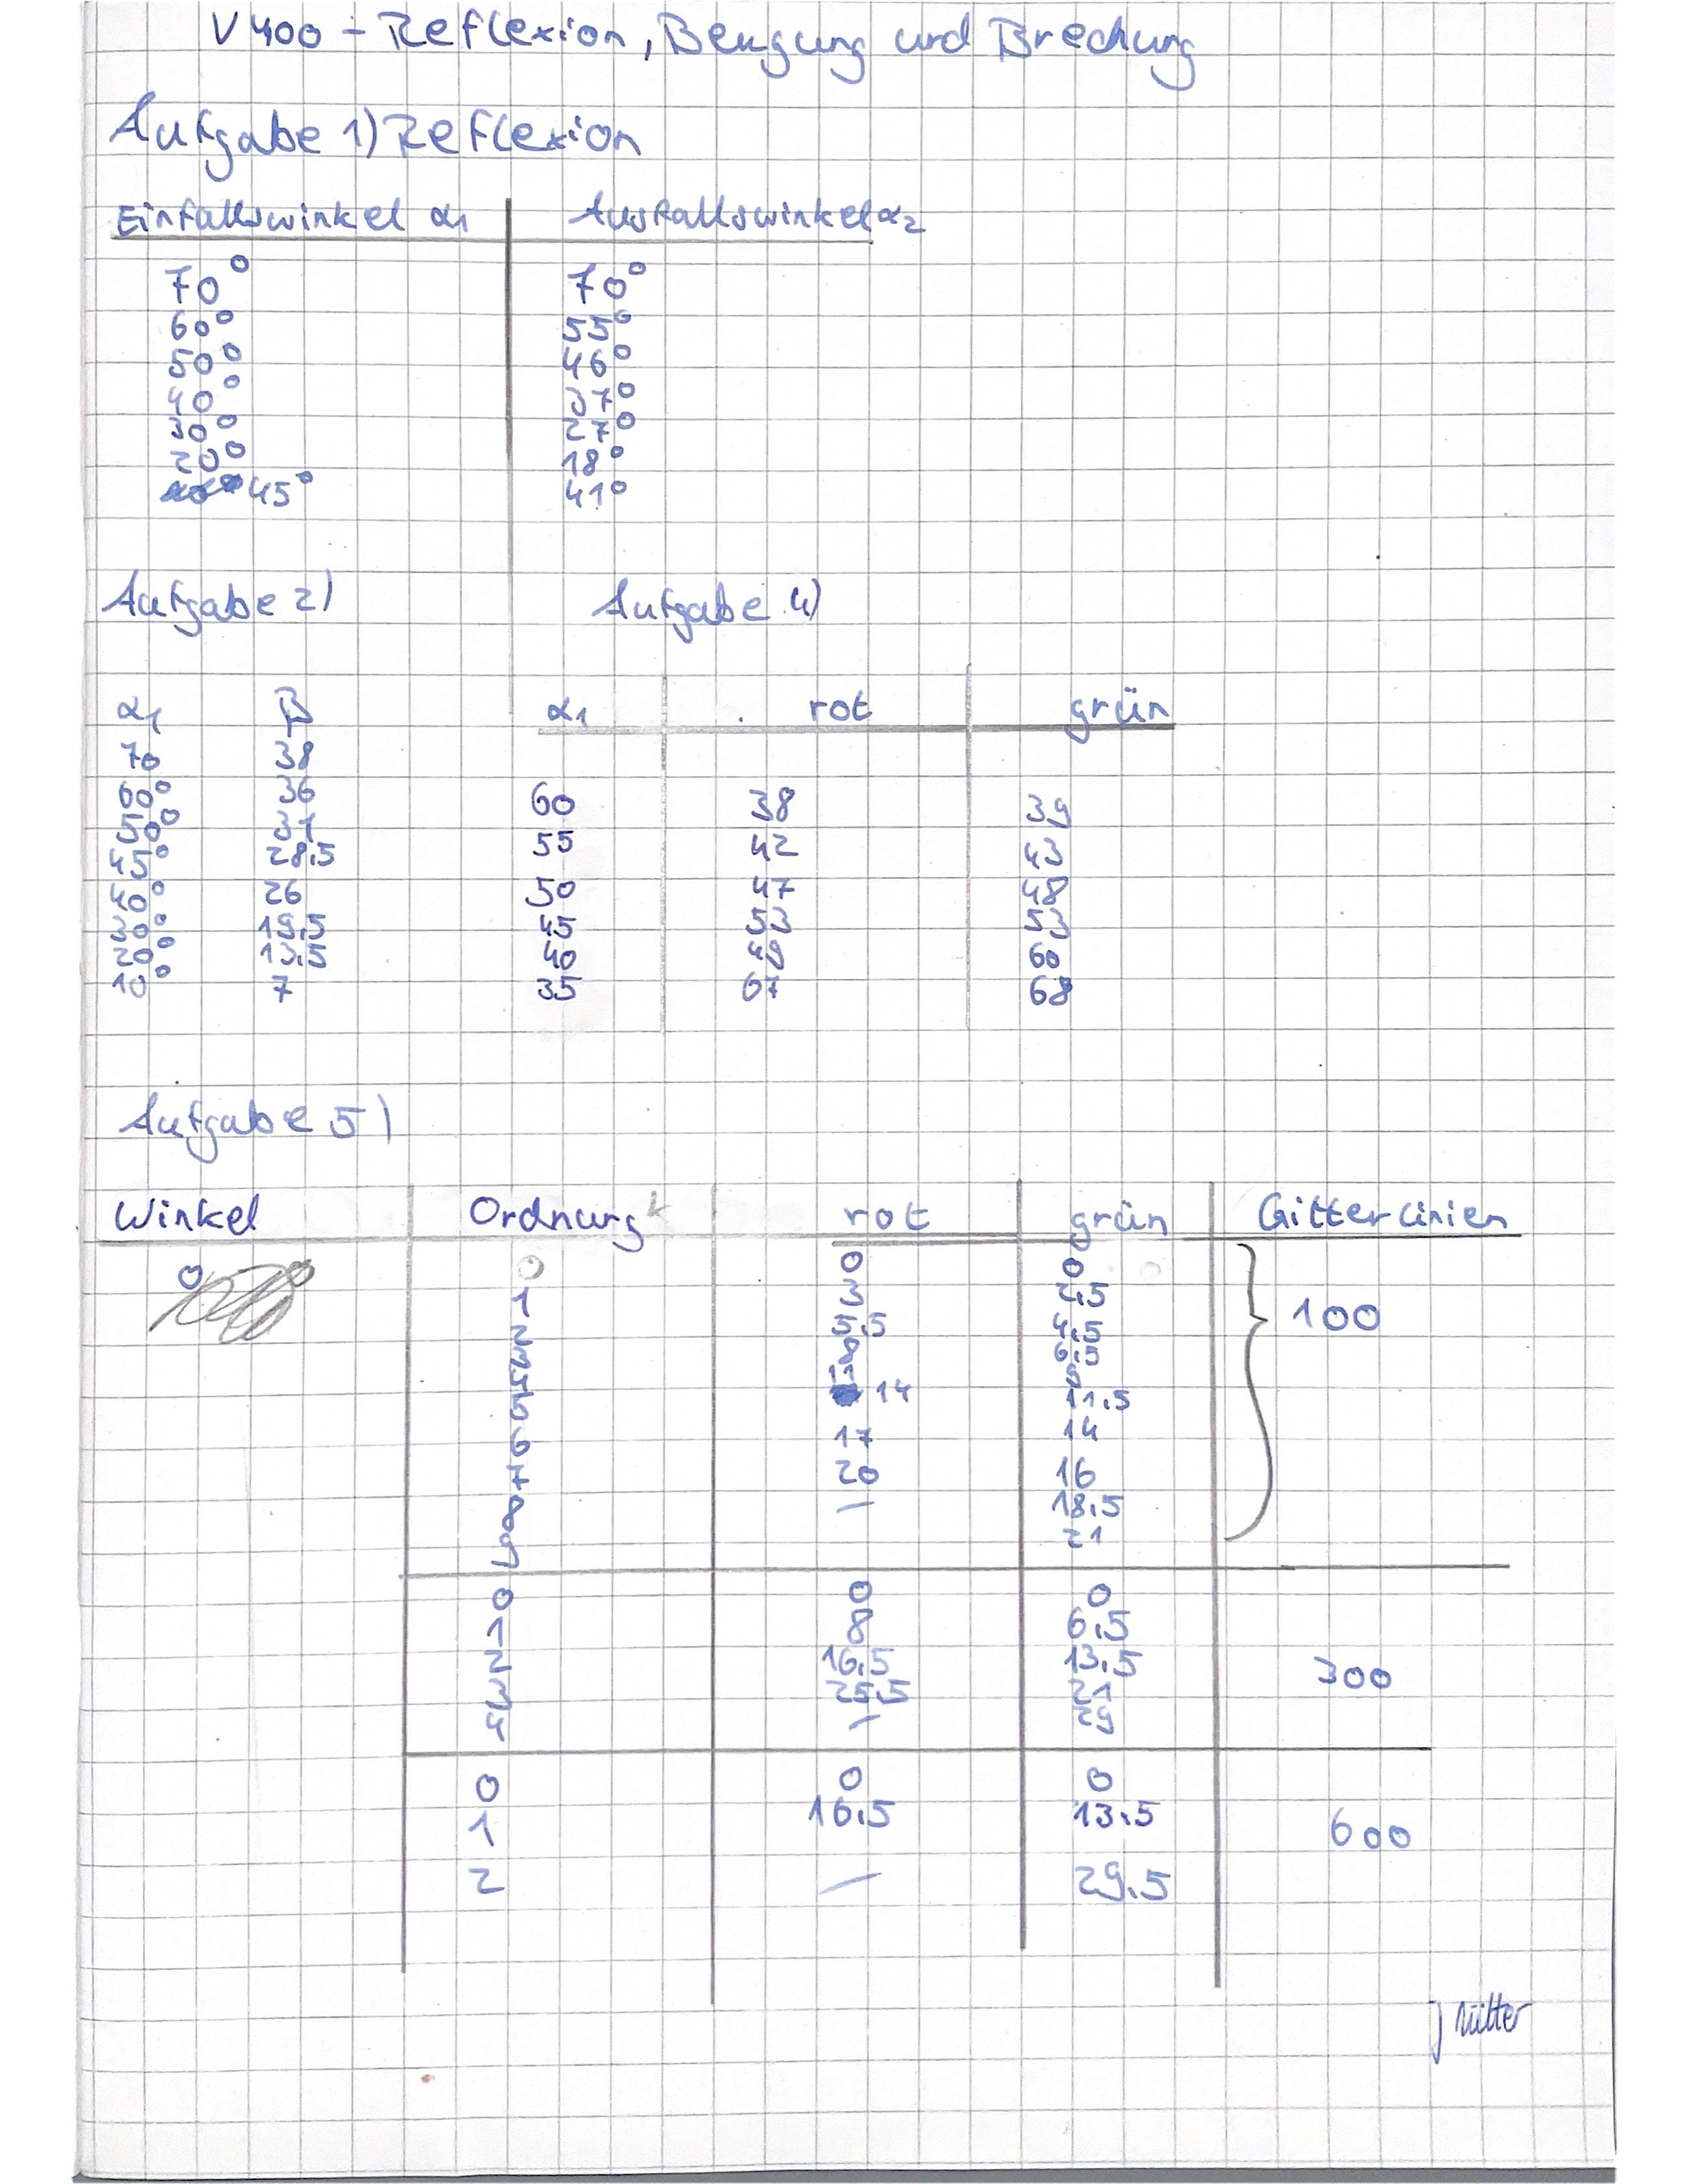
\includegraphics[width=0.7\textwidth]{data/origDaten.jpg}
  \caption{Originale Messdaten.}
  \label{fig:origDaten1}
\end{figure}